\documentclass[aspectratio=169]{beamer}
\usepackage[style=authortitle,backend=bibtex]{biblatex}
\addbibresource{references.bib}
%
% Choose how your presentation looks.
%
% For more themes, color themes and font themes, see:
% http://deic.uab.es/~iblanes/beamer_gallery/index_by_theme.html
%

\mode<presentation>
{
  \usetheme{default}      % or try Darmstadt, Madrid, Warsaw, ...
  \usecolortheme{default} % or try albatross, beaver, crane, ...
  \usefonttheme{default}  % or try serif, structurebold, ...
  \setbeamertemplate{navigation symbols}{}
  \setbeamertemplate{caption}[numbered]
} 
\addtobeamertemplate{navigation symbols}{}{%
	\usebeamerfont{footline}%
	\usebeamercolor[fg]{footline}%
	\hspace{1em}%
	\insertframenumber/\inserttotalframenumber
}

\setbeamertemplate{frametitle continuation}[from second]
%\setbeamertemplate{bibliography item}[text]
%\setbeamertemplate{navigation symbols}{}


\usepackage[english]{babel}
\usepackage[utf8]{inputenc}
\usepackage[T1]{fontenc}
\usepackage{xcolor}
\usepackage{multirow}
\usepackage{caption}
\usepackage{subcaption}
\usepackage{hyperref}
\usepackage{wrapfig}
\usepackage{placeins}
%\usepackage[table,xcdraw]{xcolor}
%\usepackage{setspace}

\newcommand\blfootnote[1]{%
	\begingroup
	\renewcommand\thefootnote{}\footnote{Picture from #1}%
	\addtocounter{footnote}{-1}%
	\endgroup
}
\newcommand\m[0]{--$\,$}
\usepackage{xpatch}
\xpatchbibmacro{cite}
{\usebibmacro{cite:title}}
{\usebibmacro{cite:title}%
	\setunit{\addcomma\space}%
	\usebibmacro{date}}
{}
{}

\newcommand{\sh}{0.2cm}
\newcommand{\wid}{7.5cm}

\title[Your Short Title]{Seminar in Robotics for CSE\\ \textcolor{red}{"GPU-based feature matching"}}
\author{Anton Maksimov\textsuperscript{1},\\ 
	supervisors: Dr. Marcin Dymczyk\textsuperscript{2,3} and Sebastian Ratz\textsuperscript{3}}
\institute{\textsuperscript{1}CSE D-MATH, \textsuperscript{2}ETH Zurich and \textsuperscript{3}Sevensense Robotics AG}
\date{16.09.2020}
\begin{document}

\begin{frame}
  \titlepage
\end{frame}

% Uncomment these lines for an automatically generated outline.
%\begin{frame}{Outline}
%  \tableofcontents
%\end{frame}

\setbeamercolor{footnote mark}{fg=blue}
\setbeamercolor{footnote}{fg=gray}
\setbeamercolor{bibliography entry author}{fg=gray}
\setbeamercolor{bibliography entry title}{fg=gray}
\setbeamercolor{bibliography entry note}{fg=gray}
\setbeamerfont{footnote}{size=\tiny}

\section{Introduction}
\begin{frame}{Introduction}
\visible<2->{\textcolor{blue}{Feature matching} is one of the most \textcolor{blue}{fundamental} techniques in computer vision:\\  image retrieval, localization and Structure-from-Motion tasks (e.g. in \texttt{maplab} package).
}

\visible<2->{
\begin{figure}
	\centering
	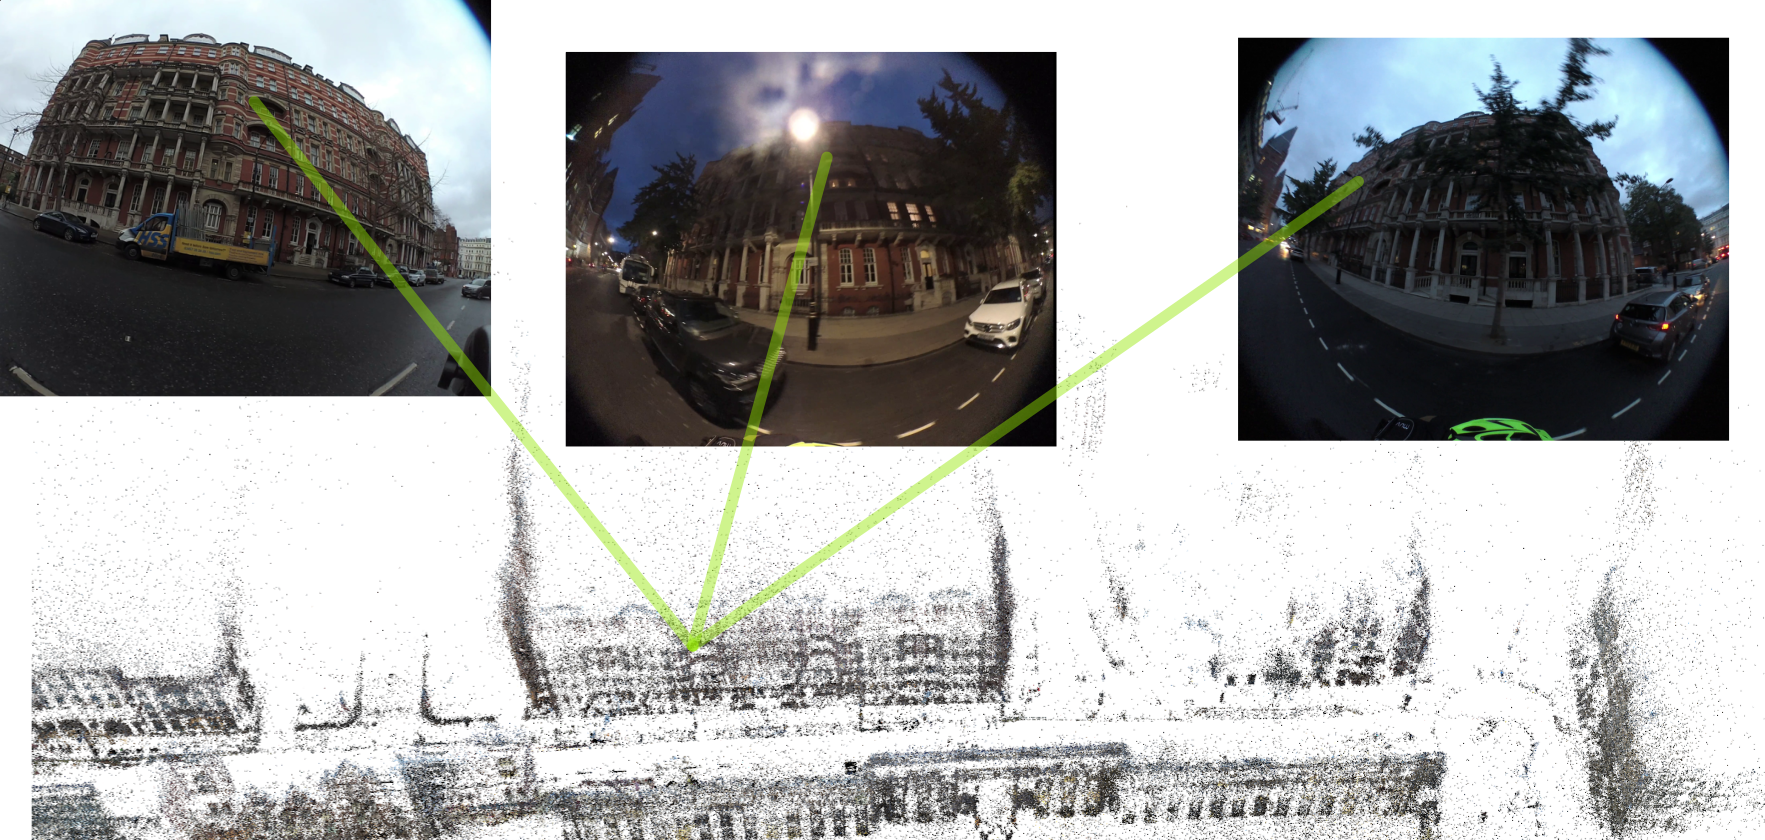
\includegraphics[width=7cm]{matching_example}
\end{figure}
}
\begin{itemize}
\visible<3->{\item \textcolor{blue}{Deep neural networks increased the quality} of matching a lot.}

\vspace{\sh}
\visible<4->{	\item However, in some applications %, such as autonomous cars, drones, virtual and augmented reality, 
the \textcolor{blue}{crucial role plays the efficiency, latency and adaptability} of the system.}

\vspace{\sh}
\visible<5->{	\item The \textcolor{blue}{modern rise of GPUs} provides the way to achieve these goals.}
\end{itemize}
\end{frame}

\section{Literature review}
\begin{frame}{Literature review}
\visible<2->{How to \textcolor{blue}{obtain} feature descriptors?
How to \textcolor{blue}{measure} their quality?
How to \textcolor{blue}{match} them?\\
}

\vspace{\sh}
\vspace{\sh}
\vspace{\sh}
\visible<3->{\centering And specifically, how to \textcolor{blue}{use GPU for efficient matching}?}
\end{frame}



\section{Feature detection and description}
\begin{frame}{}
\centering \Large How to \textcolor{blue}{obtain} descriptors?

\end{frame}

\begin{frame}{Philosophy of feature detection and description}
\begin{itemize}
	\visible<2->{\item The conventional approach -- \textcolor{blue}{detect-then-describe} $\Rightarrow$\\
	search for keypoints and producing of their descriptors are done \textcolor{blue}{sequentially} and usually \textcolor{blue}{with hand-crafted keypoints and descriptors}.
}
	
	\vspace{\sh}
	\visible<3->{\item Novel \textcolor{blue}{detect-and-describe}, in opposite, $\Rightarrow$\\
		doing these tasks \textcolor{blue}{simultaneously}, allowing of using \textcolor{blue}{more information and better consistency.}}
\end{itemize}
\visible<4->{
	\begin{figure}
		\centering
		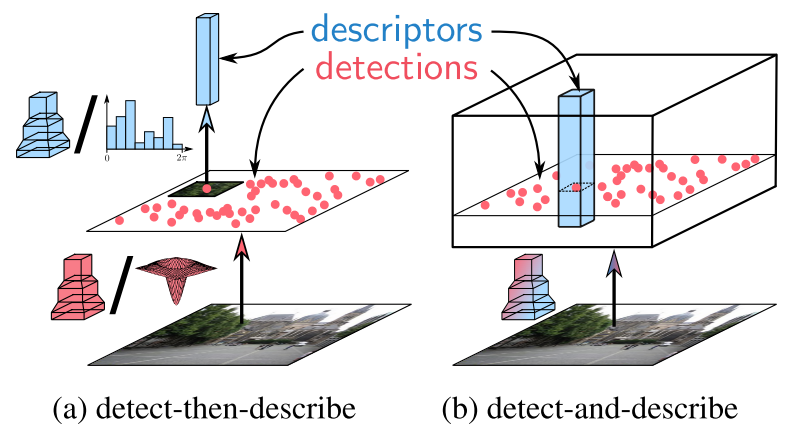
\includegraphics[width=8.5cm]{detect_describe}
	\end{figure}
}
\end{frame}

\begin{frame}{Feature detection and description}
\visible<2->{\textbf{SuperPoint}~\footcite{DeTone2018SuperPointSI}
idea: to \textcolor{blue}{pretrain feature detector} on artificially warped geometric objects.
}
\vspace{\sh}
\begin{itemize}
	\visible<3->{\item[+] Overall \textcolor{blue}{better quality of matching} than traditional methods.
	}
\vspace{\sh}
\visible<4->{\item[+] \textcolor{blue}{Fully-convolutional model}, needs one pass to compute descriptors.
}
\vspace{\sh}
	\visible<5->{\item[{--}] The \textcolor{blue}{descriptor isn't learnable and is fixed}, it constrains its efficiency.
	}
\vspace{\sh}
	\visible<6->{\item[{--}]Training on artificial examples \textcolor{blue}{introduces bias towards detecting planar geometric structures} and is worse for the real world images.
	}
\end{itemize}
\visible<2->{
\begin{figure}
	\centering
	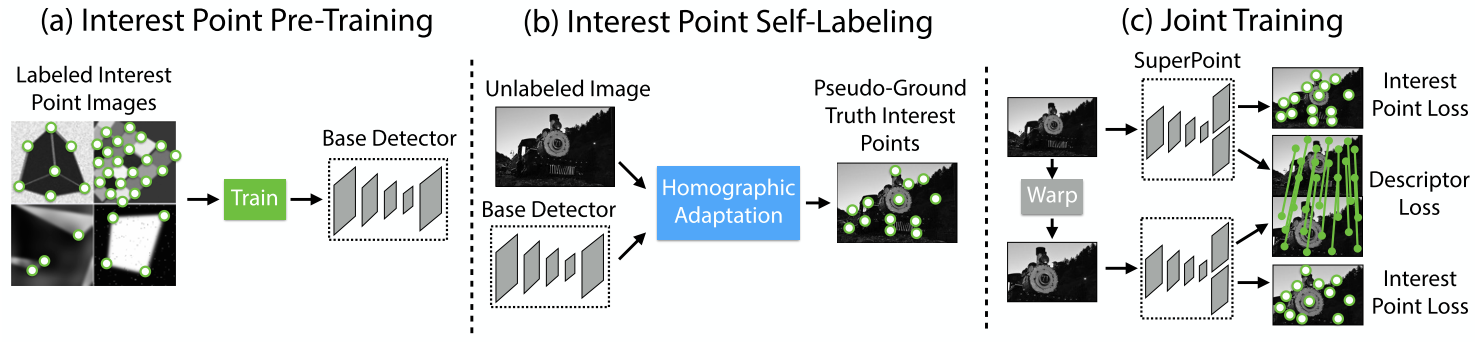
\includegraphics[width=14.5cm]{SemCSE_Superpoint}
\end{figure}
}
\end{frame}


\begin{frame}{Feature detection and description}
\textbf{D2--Net}~\footcite{Dusmanu2019D2NetAT} idea: \textcolor{blue}{joint detection and description} pipeline.
\begin{itemize}
	\visible<2->{\item[+] Was shown to be \textcolor{blue}{consistently better than SuperPoint and the previous ones}.
	}
	\visible<3->{\item[--] Predicts properties of keypoints in rather \textcolor{blue}{empiric conventional fashion}\\
	(softmax, non-maximum suppression among descriptors).
	}
\end{itemize}

\begin{figure}
	\centering
	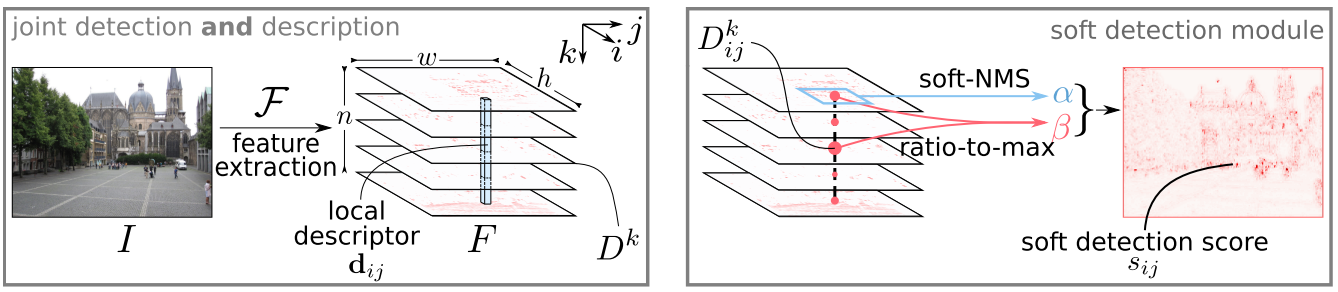
\includegraphics[width=15.0cm]{SemCSE_D2}
\end{figure}

\end{frame}


\begin{frame}{Feature detection and description}
\textbf{R2D2}~\footcite{R2D2} idea: estimate separately \textcolor{blue}{reliability} and \textcolor{blue}{repeatability} of descriptors
\begin{itemize}
	\visible<2->{\item[+] The quality of matching is \textcolor{blue}{at the level or better} than others.
	}
	\visible<3->{\item[+]\textcolor{blue}{The model is more compact}, as its descriptor length and the number of weights is much less than what the competitors have.
	}
	\visible<4->{\item[--] Needs the \textcolor{blue}{choice of higher number of hyperparameters}.
	}
\end{itemize}
\begin{figure}
	\centering
	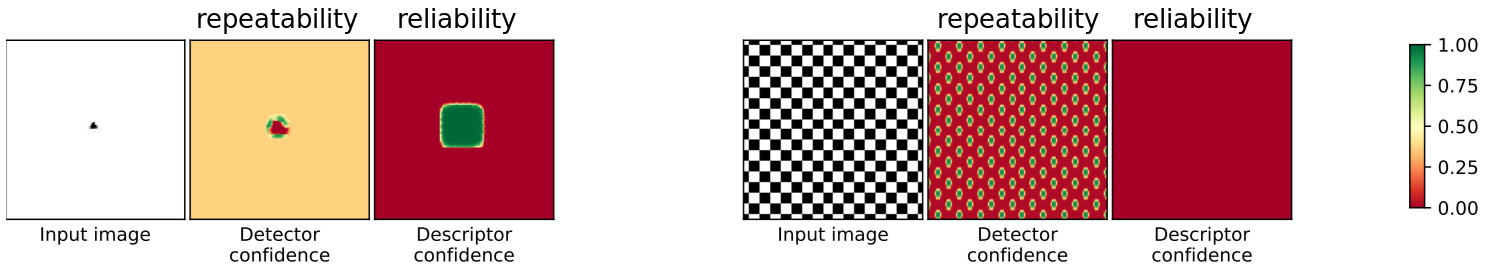
\includegraphics[width=15.0cm]{SemCSE_R2D2_edited}
\end{figure}

\end{frame}


\begin{frame}{Feature detection and description}
\textbf{UR2KiD}~\footcite{yang2020ur2kid} idea: \textcolor{blue}{multi-task} for local (patches) and global (image retrieval) description.
\begin{itemize}
	\visible<2->{\item[+] Is more \textcolor{blue}{robust against appearance and scale changes} than the previous methods. 
	}
	\visible<3->{\item[+] Its idea of \textcolor{blue}{multi--task learning leads for the improvement in both tasks} and \textcolor{blue}{could be useful in the future} constructions of weakly supervised but powerful networks.
	}
\end{itemize}
\begin{figure}
	\centering
	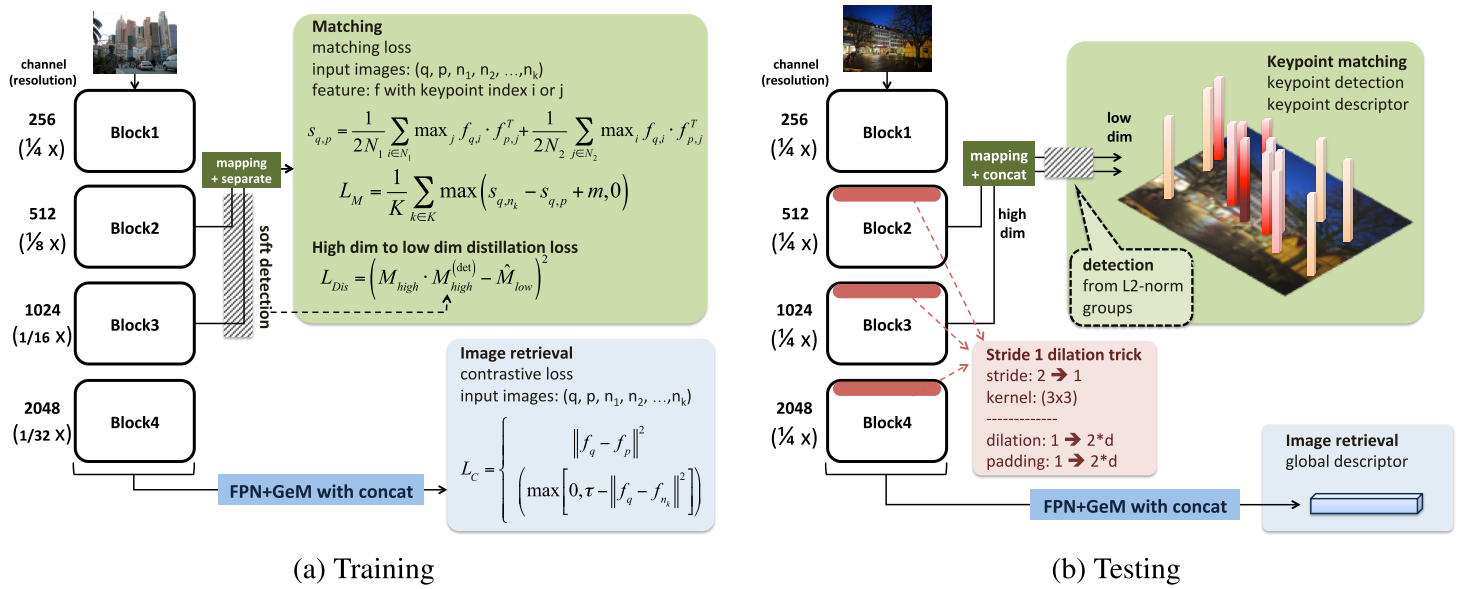
\includegraphics[width=12.5cm]{SemCSE_UR2KID}
\end{figure}
\end{frame}

\section{Descriptors quality assessment}
\begin{frame}

\centering \Large We observed descriptors construction.\\

\vspace{\sh}
\visible<2->{\centering \Large How to measure their \textcolor{blue}{quality}?}
\end{frame}


\begin{frame}{Descriptors quality assessment}
\textbf{HPatches}~\footcite{HPatches} --- dataset for \textbf{2D--2D matching} assessment.\\
Consists of \textcolor{blue}{extracted and augmented with noise and transformations patches} from various image sequences in varying lightning conditions and camera positions.

\begin{figure}
	%\centering
	\begin{minipage}[b]{5cm}
		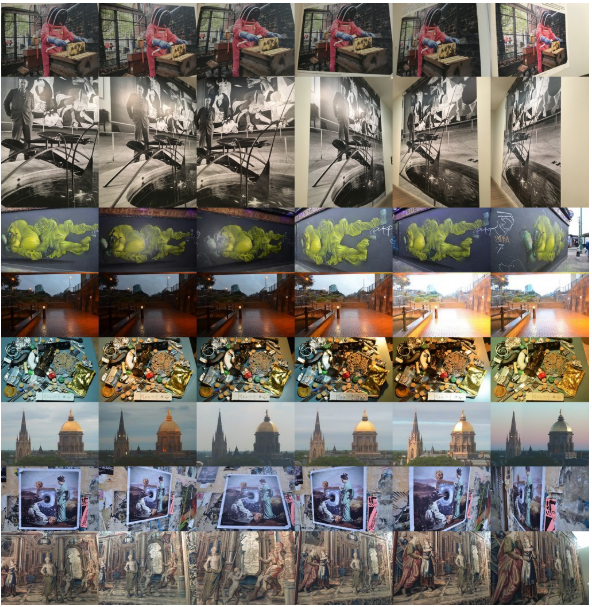
\includegraphics[width=5cm]{SemCSE_hpatches}
	\end{minipage}%
	\hfill
	\begin{minipage}[b]{5cm}
		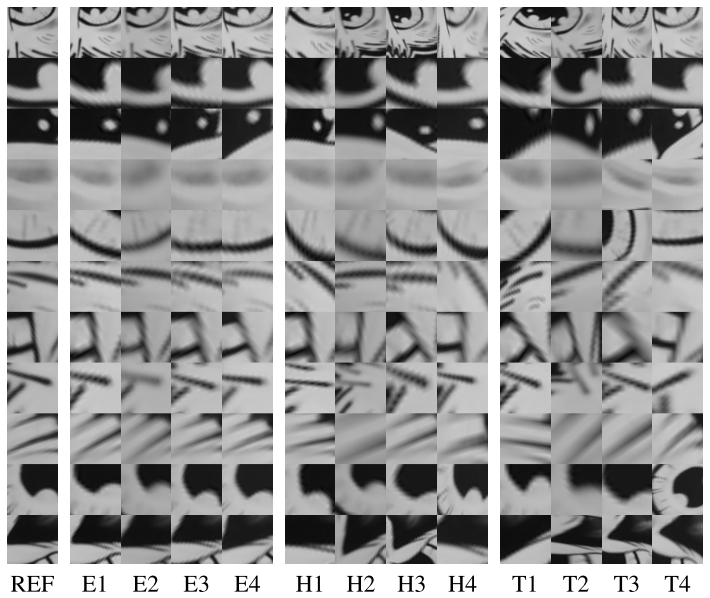
\includegraphics[width=5cm]{SemCSE_hpatches2}
	\end{minipage}%
\end{figure}

\end{frame}


\begin{frame}{Descriptors quality assessment}
\textbf{The Long--Term Visual Localization Benchmark} \footcite{visual_loc}  consists of several datasets of \textcolor{blue}{scenes under different appearance conditions} for the \textbf{2D--3D} problem of estimating the 6 DoF camera pose.
\begin{figure}
\centering
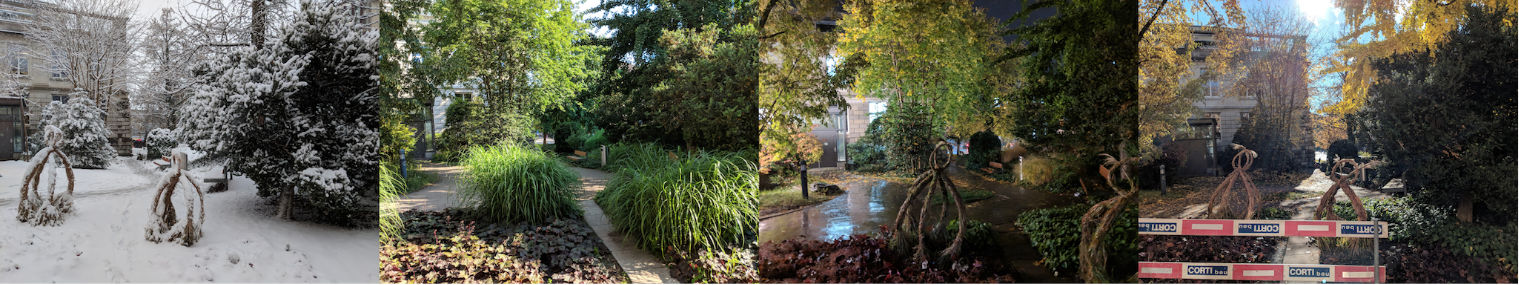
\includegraphics[width=13cm]{SemCSE_longterm}
\end{figure}
\end{frame}


\section{Matching of features}
\begin{frame}
\centering \Large We observed how to \textcolor{blue}{construct good descriptors}.\\
\vspace{\sh}
\vspace{\sh}
\vspace{\sh}
\vspace{\sh}
\visible<2->{\centering \Large How to \textcolor{blue}{match} them finally?}
\end{frame}


\begin{frame}{Matching of features}
\hspace{-0.5cm}\textbf{Hierarchical Feature Network}~\footcite{Sarlin2019b} idea: \textcolor{blue}{coarse-to-fine} pose estimation with \textcolor{blue}{distillation}.
\begin{itemize}
	\visible<2->{\item[+] \textcolor{blue}{Outperformed competitors} of the time on large-scale benchmarks with substantial appearance changes.
	}
	\visible<3->{\item[+] \textcolor{blue}{Distillation allows to improve the method} using the global teacher signal.
	}
	\visible<4->{\item[+] Simultaneously \textcolor{blue}{estimates the camera 6-DoF pose}.
	}
	\visible<5->{\item[{$\pm$}] \textcolor{blue}{Tailored for mobile} low computational power applications.
	}
\end{itemize}
\begin{figure}
	\centering
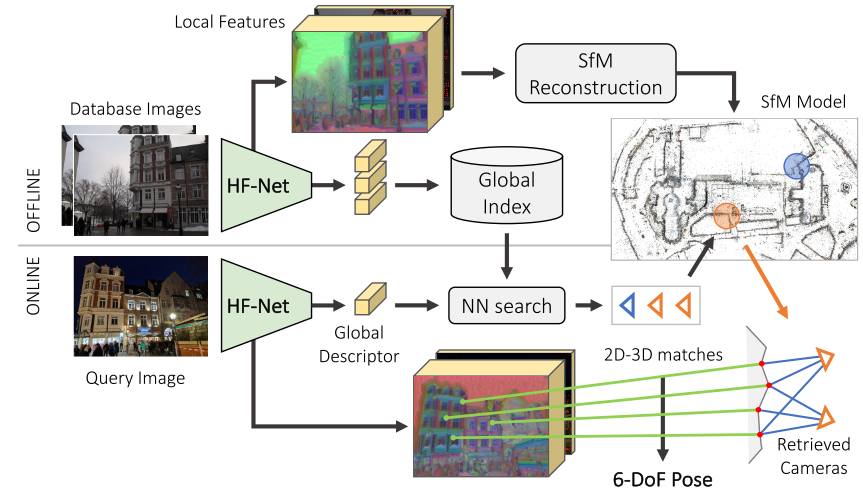
\includegraphics[width=7.5cm]{SemCSE_HF}
\end{figure}
\end{frame}


\begin{frame}{Matching of features}
\textbf{Order--aware network}~\footcite{Zhang2019} idea: use \textcolor{blue}{local context} and feature \textcolor{blue}{permutation invariance}.\\
\begin{itemize}
	\visible<2->{\item[+] Shows \textcolor{blue}{better performance} than the other contemporary ones%, including extensions of the PointNet structure
	}
	\visible<3->{\item[+] Captures \textcolor{blue}{both global and local context}.
	}
	\visible<4->{\item[{--}] \textcolor{blue}{Relies heavily on the quality of descriptors}, as it is an outlier--rejection network uses the nearest--neighbor search.
	}
\end{itemize}

\begin{figure}
	\centering
	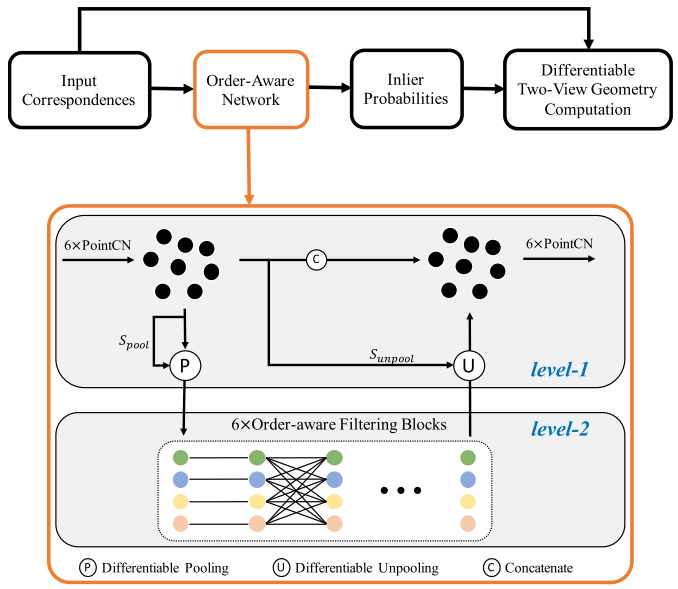
\includegraphics[width=5.5cm]{SemCSE_OA}
\end{figure}
\end{frame}


\begin{frame}{Matching of features}
\textbf{SuperGlue}~\footcite{Sarlin2019a} idea: 
use a
\textcolor{blue}{graph neural network and attention} to solve an assignment
optimization problem.
\begin{itemize}
	\visible<2->{\item[+] \textcolor{blue}{Achieves significant improvement} over existing approaches, working \textcolor{blue}{real--time} and \textcolor{blue}{well both with learned and traditional features}.
	} 
\end{itemize}

\begin{figure}
	\centering
	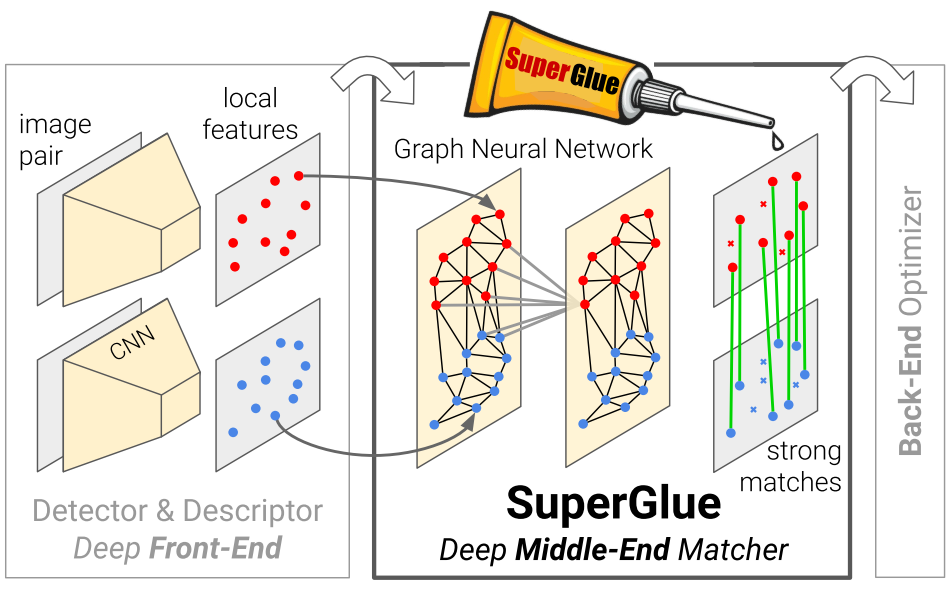
\includegraphics[width=8.0cm]{SemCSE_Superglue}
\end{figure}

\end{frame}

\section{GPU-based approaches}
\begin{frame}

\centering \Large How to \textcolor{blue}{leverage GPU} for more efficient matching?\\
(e.g. with huge databases)
\end{frame}


\begin{frame}{GPU-based approaches}
Nagy et al.\footcite{GPU_VIO} describe GPU--based \textbf{acceleration for visual--inertial odometry}.\\
\visible<2->{Idea: \textcolor{blue}{optimize on the low--level the most prominent for latency operations}: non--maximum suppression and consequent feature selection.
}
\begin{itemize}
	\visible<3->{\item[+] \textcolor{blue}{Much faster} than competitors.
	}
	\visible<4->{\item[$\pm$] \textcolor{blue}{Uniform distribution} of features. 
	}
\end{itemize}
\begin{figure}
	\centering
	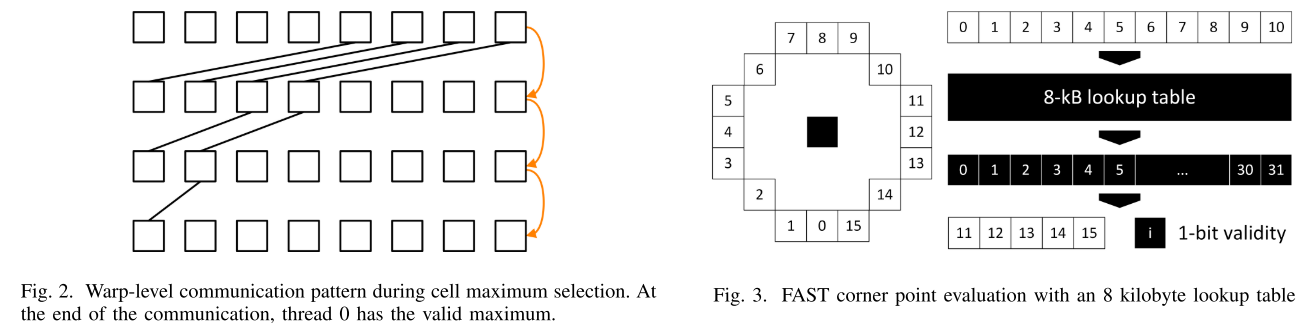
\includegraphics[width=15.0cm]{SemCSE_vio}
\end{figure}
\end{frame}


\begin{frame}{GPU-based approaches}
\textbf{Cascade Hashing}~\footcite{cascade_hashing} idea: reduce number of candidates by hierarchical space hashing.\\
\visible<2->{\textcolor{blue}{Dissects space multiple times} with random planes and \textcolor{blue}{binary encodes} descriptors by containing in one or another half-spaces.
}
%It uses nested hashes obtained by dissecting the multi--dimensional feature space with random planes and decoding every bit of hash as a corresponding side of the plane.
\begin{itemize}
	\visible<3->{\item[+] \textcolor{blue}{Much faster} than competitors.
	} 
	\visible<4->{\item[+] \textcolor{blue}{Robust to noise, unsupervised.}
	}
\end{itemize}
\begin{figure}
	\centering
	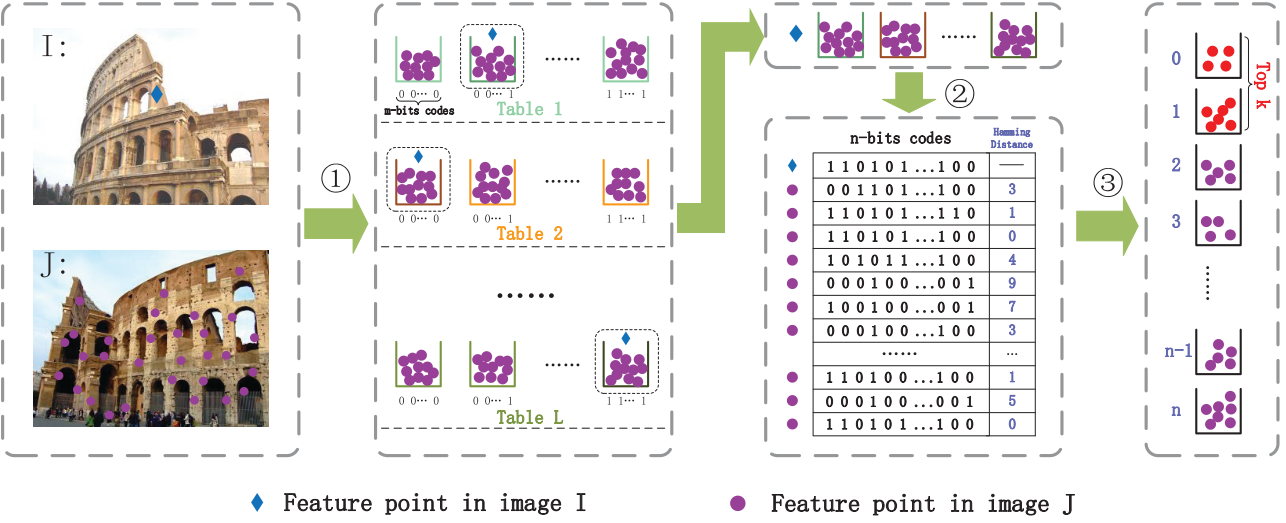
\includegraphics[width=12.0cm]{SemCSE_cascade_hashing}
\end{figure}
\end{frame}

\section{Practical part}
\begin{frame}{Literature $\Rightarrow$ experience in reality}
\visible<2->{\noindent\textbf{General problem:} \textcolor{blue}{matching descriptors} from 2D image to 3D database or between two images. This is the \textcolor{blue}{fundamental operation} in computer vision.\\
}
\visible<3->{
	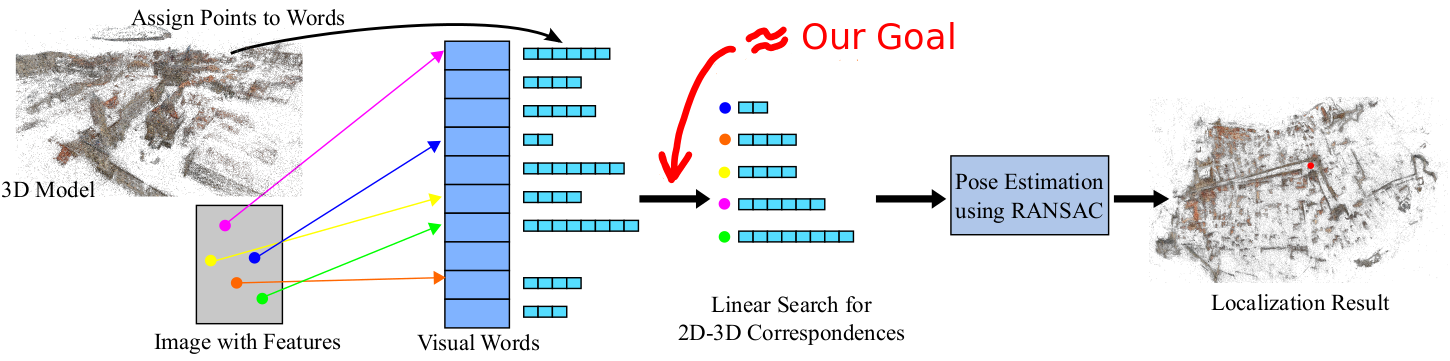
\includegraphics[width=14.0cm]{Descriptors_2}
%\captionof{figure}{Double log graph}

}
\visible<4->{
\vspace{\sh}
\textbf{Idea:} $\bullet$ to \textcolor{blue}{try different methods} for finding the \textcolor{blue}{nearest--neighbor} for descriptors,\\ \hspace{1cm}$\bullet$ \textcolor{blue}{compare CPU and GPU} versions.\\
}
\visible<5->{
\vspace{\sh}
\textbf{Formulation:} we have $N\in \mathbb{R}^F$ \textcolor{blue}{query descriptors} and $N_{\text{db}}\in \mathbb{R}^F$ \textcolor{blue}{database descriptors}.\\
}
\visible<6->{
\vspace{\sh}
\textbf{Goal:} \textcolor{blue}{find the closest descriptor in DB} (in Euclidean metric) for each one in the query. 
}
\end{frame}


\begin{frame}{Methods compared}
\begin{enumerate}
	\visible<2->{\item \textcolor{blue}{Brute--force:} \textbf{check all  distances} ($N\cdot N_{\text{db}}$) and find the closest to each of the query descriptors among the DB ones.
}
	\vspace{\sh}
	\visible<3->{\item Further methods %(called in general as "hashing") 
		\textcolor{blue}{use encodings} $\mathbf{h}_i$ of descriptors as a \textcolor{blue}{binned} % by $W$~
		\textcolor{blue}{distances to the set of random %$M$~
		planes}. %s, whose normals $\mathbf{a}_i$ are normally distributed, and shifts $\mathbf{b}_i$ are uniformly distributed.
}
\visible<4->{
	\begin{equation*}
	h_{i,\,j} = \Bigl\lfloor\frac{\mathbf{a}_j\cdot \mathbf{d}_i + \mathbf{b}_j}{W}\Bigr\rfloor, \;\; 
	\text{where } \mathbf{a}_j \sim \mathcal{N}(0, 1)^{M \times F}, \:
	\mathbf{b}_j \sim \text{Unif}(0, W)
	\end{equation*}
}
\begin{enumerate}

\visible<5->{	
	\item \textcolor{blue}{"Manhattan check in encoded space":} candidates to check are chosen by the \textbf{closest encodings in Manhattan distance}. %, then the closest one among them is found using Euclidean distance.
}	
	
\visible<6->{	
	\vspace{\sh}
	\item \textcolor{blue}{Locally Sensitive Hashing (LSH)~\footcite{Shakhnarovich2005NearestNeighborMI}:}
	obtained \textbf{binned encodings are hashed} using polynomial hashing several times. % mod $tableSize$. The procedure is repeated $L$ times. 
	\textbf{For faster search of hits linked lists (chaining)} of DB occurrences by their value are used.%in $[0, \ldots, tableSize]$ 
} 


\end{enumerate}
\visible<7->{For these two methods we use empirically the most reasonable parameters.
}
\end{enumerate}


\end{frame}



\section{Efficiency plots}
\begin{frame}{Time depending on algorithm, machine and \textbf{query} size ($N_{\text{db}} \approx 28\text{K}$)}
\begin{figure}
	\centering

	\begin{minipage}{8.0cm}
		
		%\caption{Time depending on algorithm/machine and query size}
		%\hspace{-1cm}
		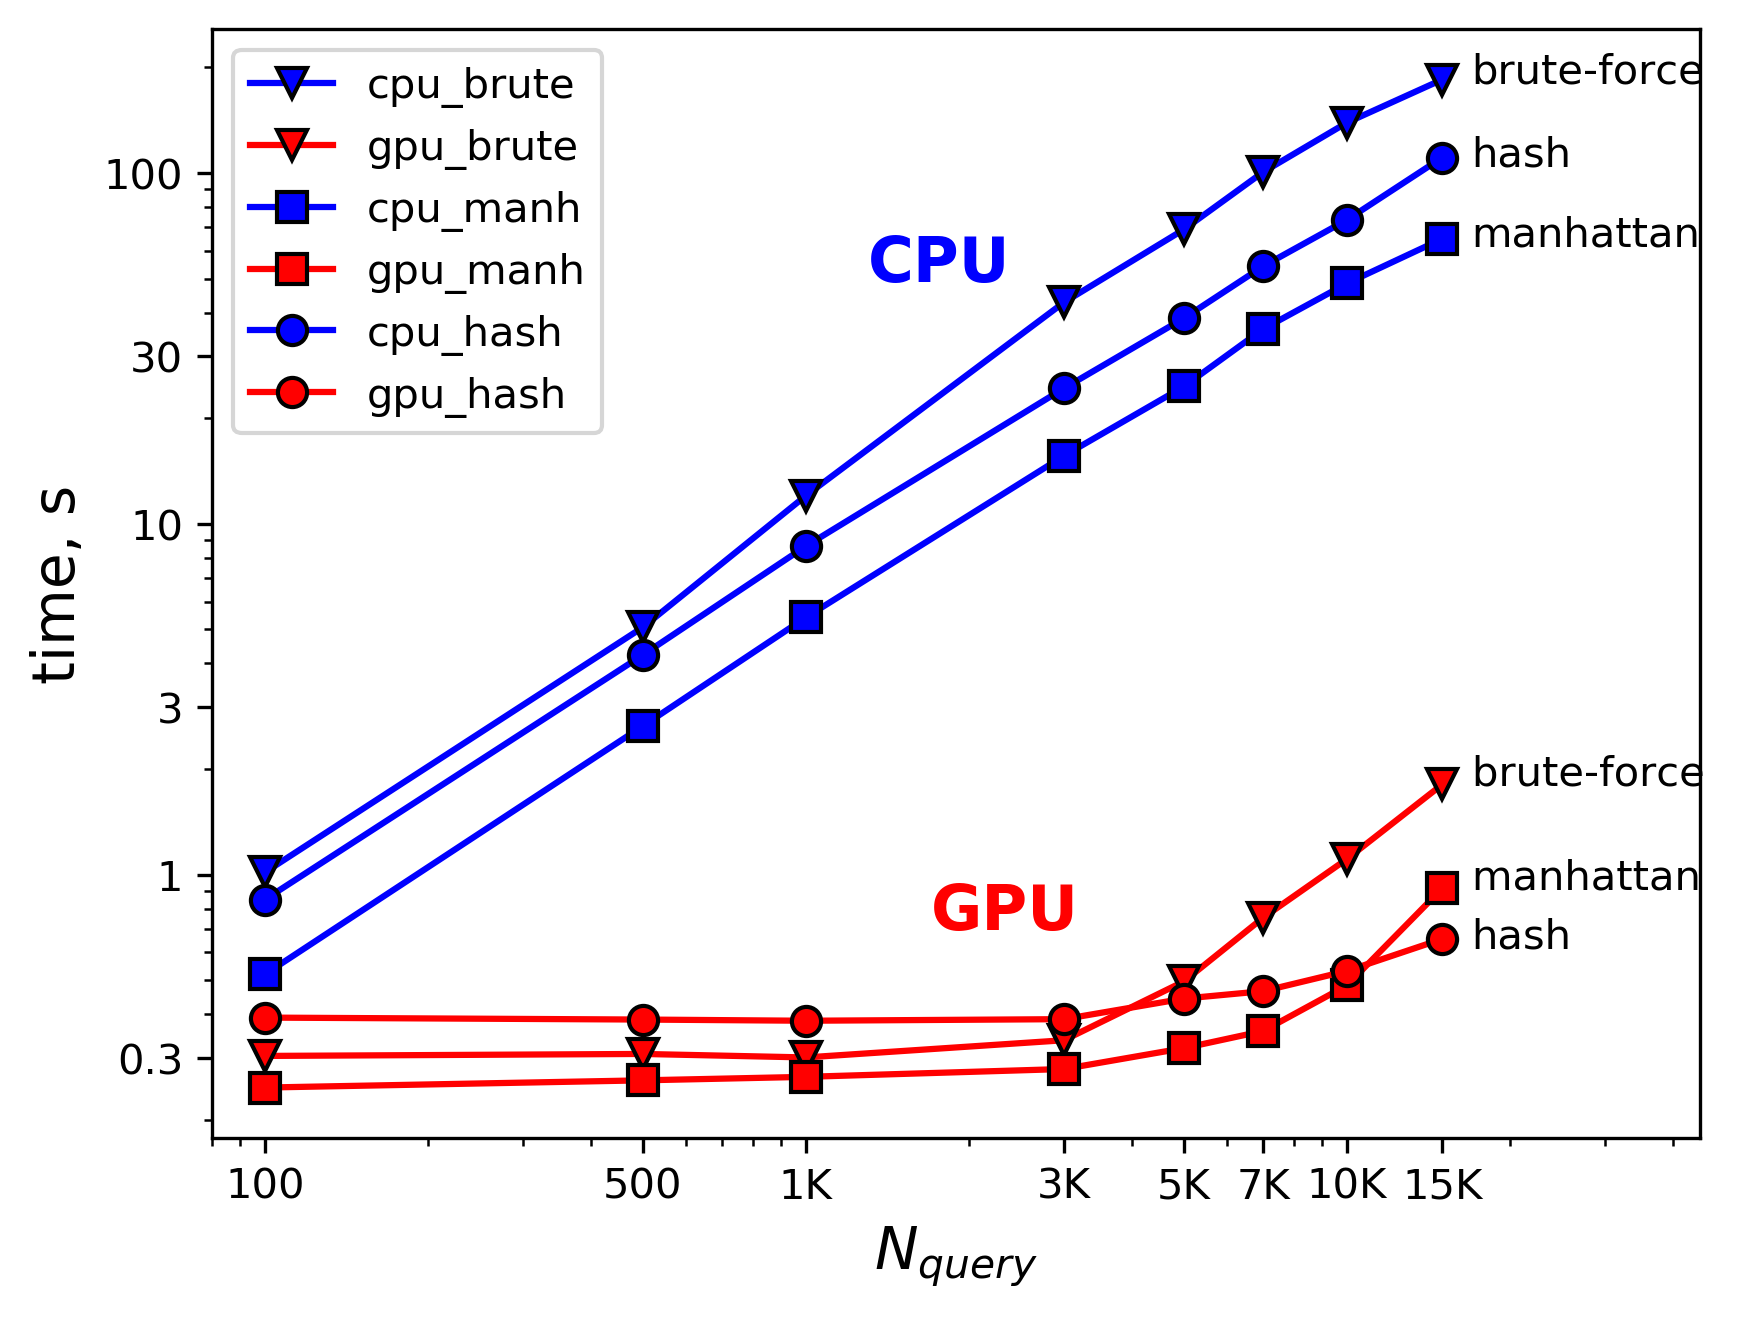
\includegraphics[width=8.0cm]{log_yx_query.png}
		
		\label{fig:test2}
	\end{minipage}
\end{figure}
\begin{itemize}
\visible<2->{
	\item \textcolor{blue}{GPU is much faster than CPU}, esp. when big query -- 2 orders change.
}
\visible<3->{
	\item \textcolor{blue}{Difference between algorithms is not so big}, it depends on parameters.
}
\visible<4->{
	\item Possible explanation for \textcolor{blue}{blow-up of GPU with big queries} - GPU memory overload.
}
\end{itemize}
\end{frame}


\begin{frame}{Sweep over different DB sizes with constant query ($N_{\text{query}} = 5\text{K}$)}
\begin{figure}
	\centering
	
	\begin{minipage}{8.0cm}
		
		%\caption{Time depending on algorithm/machine and query size}
		%\hspace{-1cm}
		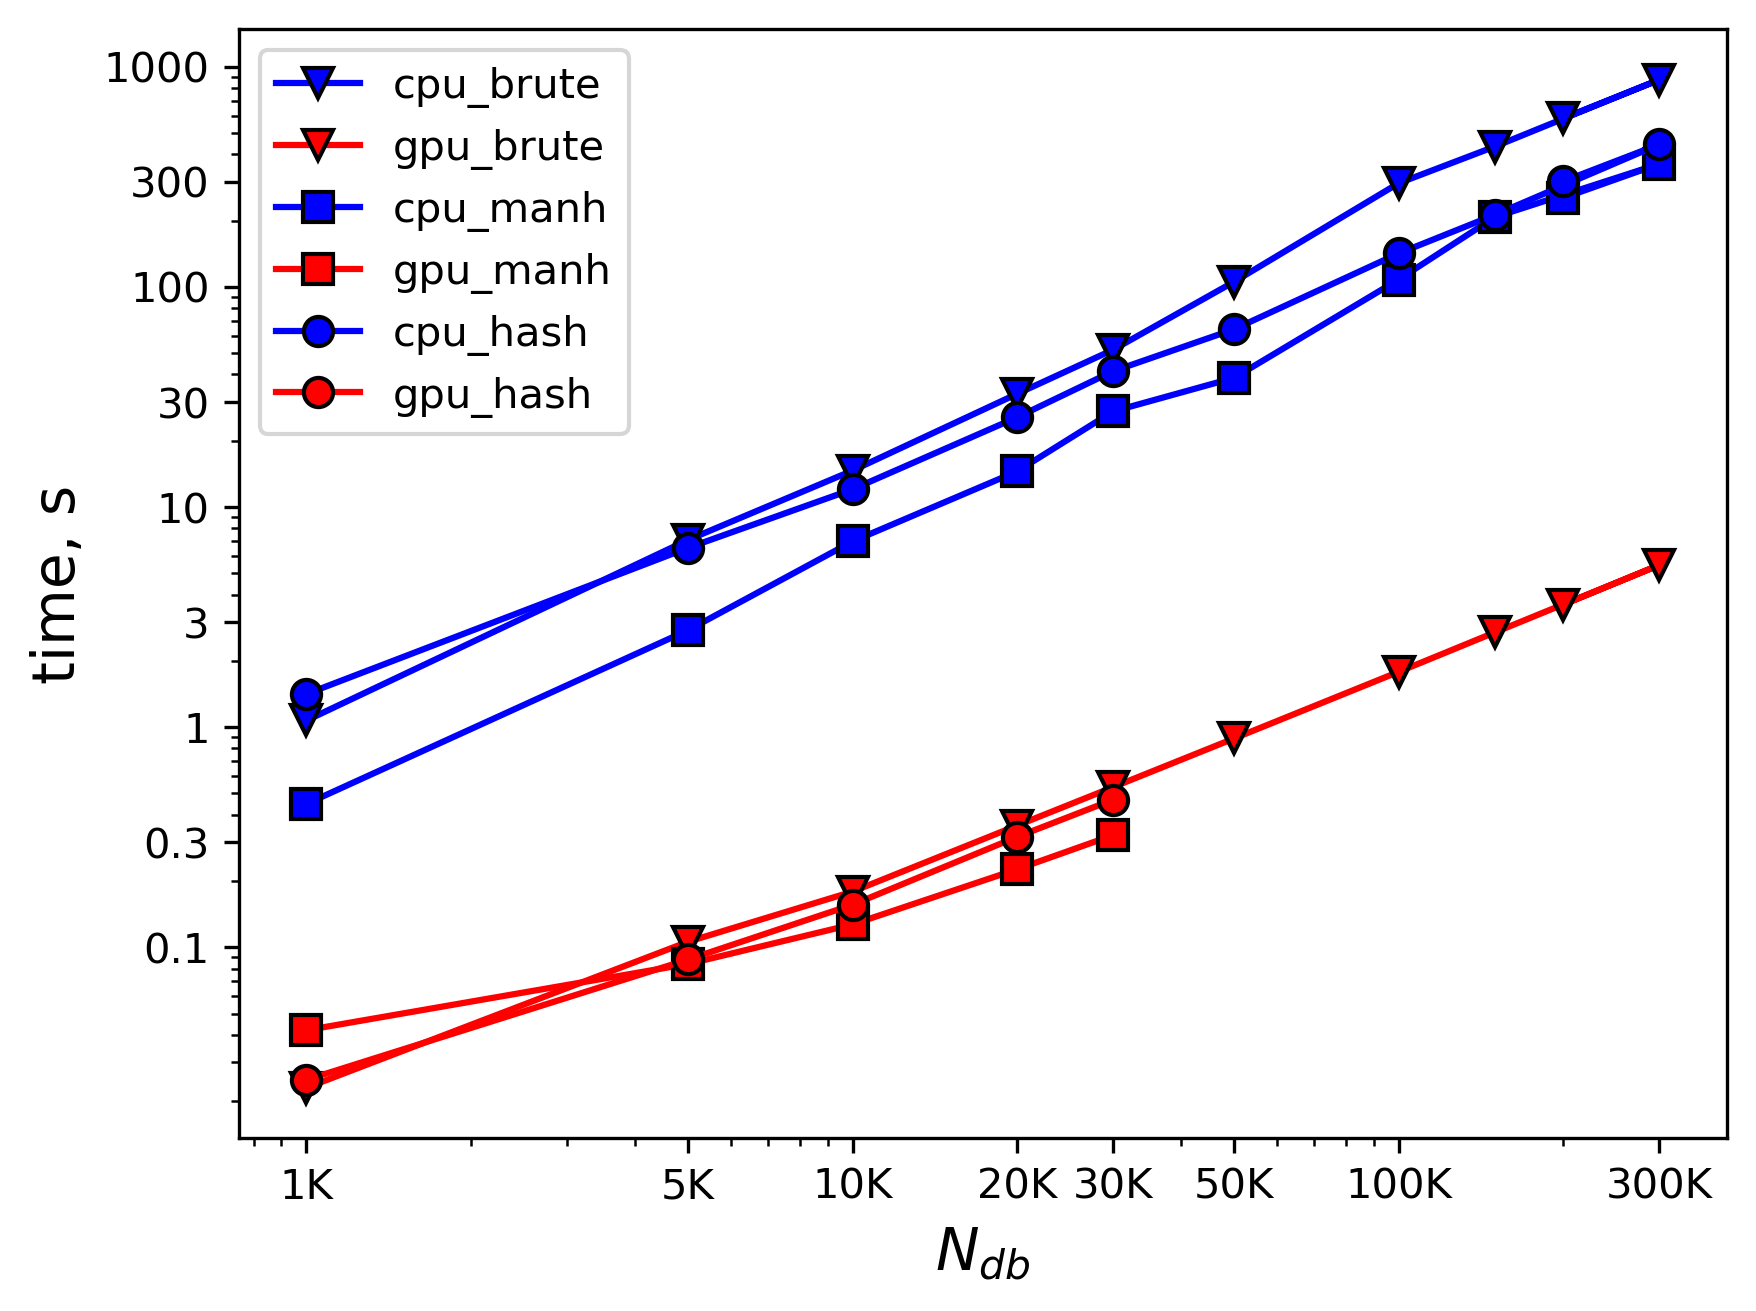
\includegraphics[width=8.0cm]{log_yx_db.png}
	\end{minipage}
\end{figure}
\begin{itemize}
\visible<2->{	
	\item \textcolor{blue}{Perfect linear} time dependency for both CPU and GPU, as expected.
}
	%\item \textcolor{red}{GPU in "hash" and "manhattan" doesn't work with more than 30K in db - too much memory needed, probably. Possible solution with "hash" (LSH) could be double--hashing --- to hash encoding of the descriptor and store hash, which is less than 128.} 
\end{itemize}
\end{frame}

\if0
\section{Visualization of correspondences}

\begin{frame}{Visualization of correspondences}
\begin{figure}
	\centering
	\begin{minipage}{10.0cm}
		
		%\caption{Time depending on algorithm/machine and query size}
		%\hspace{-1cm}
		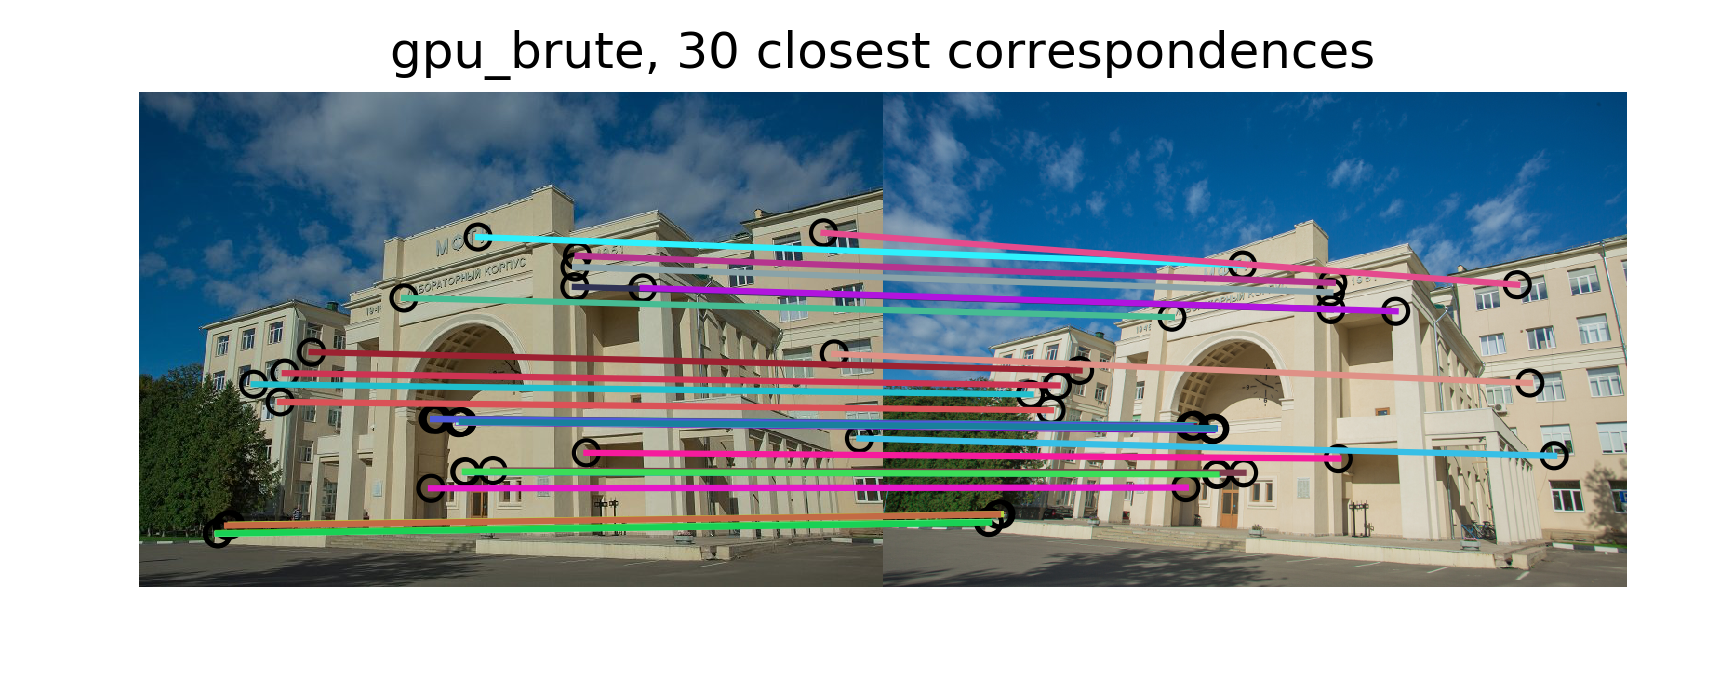
\includegraphics[width=10.0cm]{corresp_gpu_brute.png}
	\end{minipage}
	\vfill
	\visible<2->{
	\begin{minipage}{10.0cm}
		
		%\caption{Time depending on algorithm/machine and query size}
		%\hspace{-1cm}
		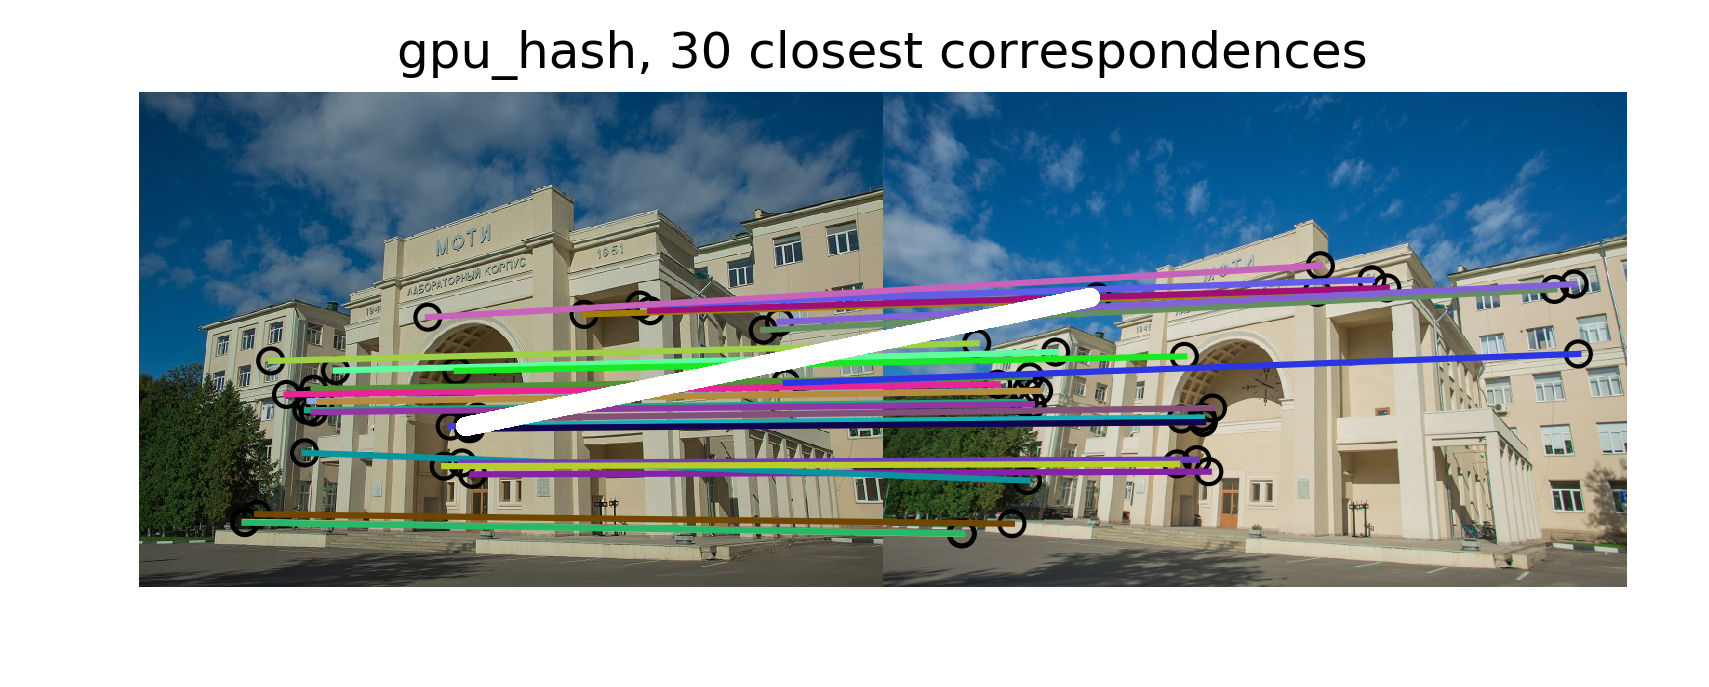
\includegraphics[width=10.0cm]{corresp_gpu_hash_edited.png}
	\end{minipage}
}
\end{figure}
\end{frame}
\fi
\section{Resume}
\begin{frame}{Resume}
\begin{table}[]
	\begin{tabular}{p{8cm}p{6cm}}
			\begin{itemize}
				\visible<2->{\item GPU allows \textcolor{blue}{to speed up} the CPU matching by \textcolor{blue}{up to 2 orders} magnitude.
							}
				\visible<3->{\item Hashing in our experiments \textcolor{blue}{can't achieve both better speed and the very same quality} of matching as GPU brute-force.
							}
				\visible<5->{\item Possible \textcolor{blue}{low-level tweaks could speed it up} potentially.
							}
				\visible<6->{\item \textcolor{blue}{Hashing is very flexible} with several parameters to tune.
							}
				\visible<7->{\item Hashing could be \textcolor{blue}{useful when speed is more important than quality} or memory constraints exist. 
							}
				\visible<8->{\item Parameter \textcolor{blue}{tuning is not obvious} for hashing. 
							}
		\end{itemize}
		
			&
			\visible<4->{\raisebox{-\totalheight}{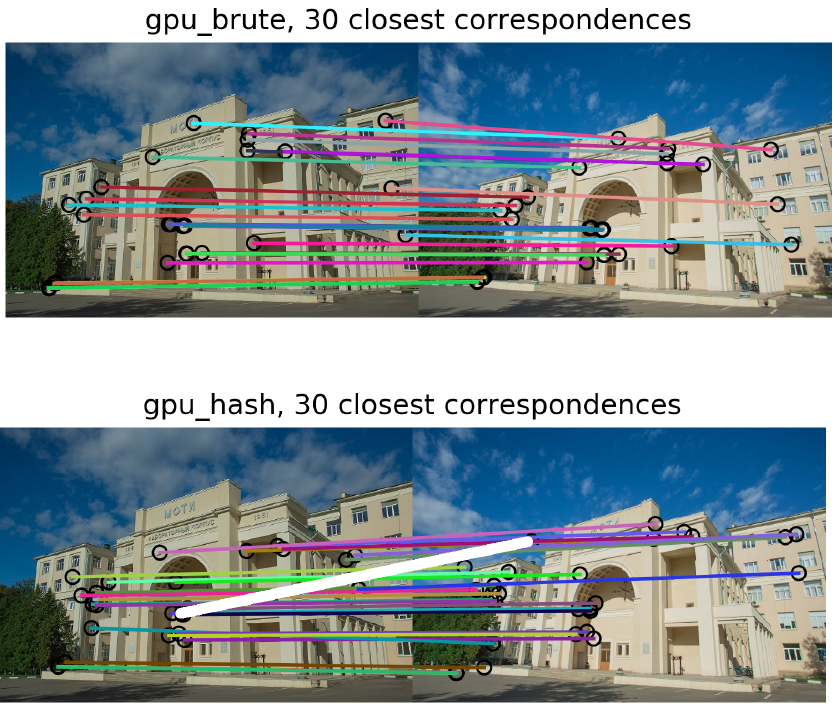
\includegraphics[width=6cm]{corresp_two}}
			}\\
		
	\end{tabular}
\end{table}

\end{frame}

%c\includegraphics[width=0.3\textwidth, height=60mm]{images/myLboro.png}}

\begin{frame}
\centering \LARGE
\vspace{0.5cm}
Questions?

\textcolor{red}{%-- To check work on different images?\\
%-- Use several different queries in a row to check that it doesn't cache?\\
}
\end{frame}

\begin{frame}
\begin{figure}
	\centering
	\begin{minipage}{\wid}
		
		%\caption{Time depending on algorithm/machine and query size}
		%\hspace{-1cm}
		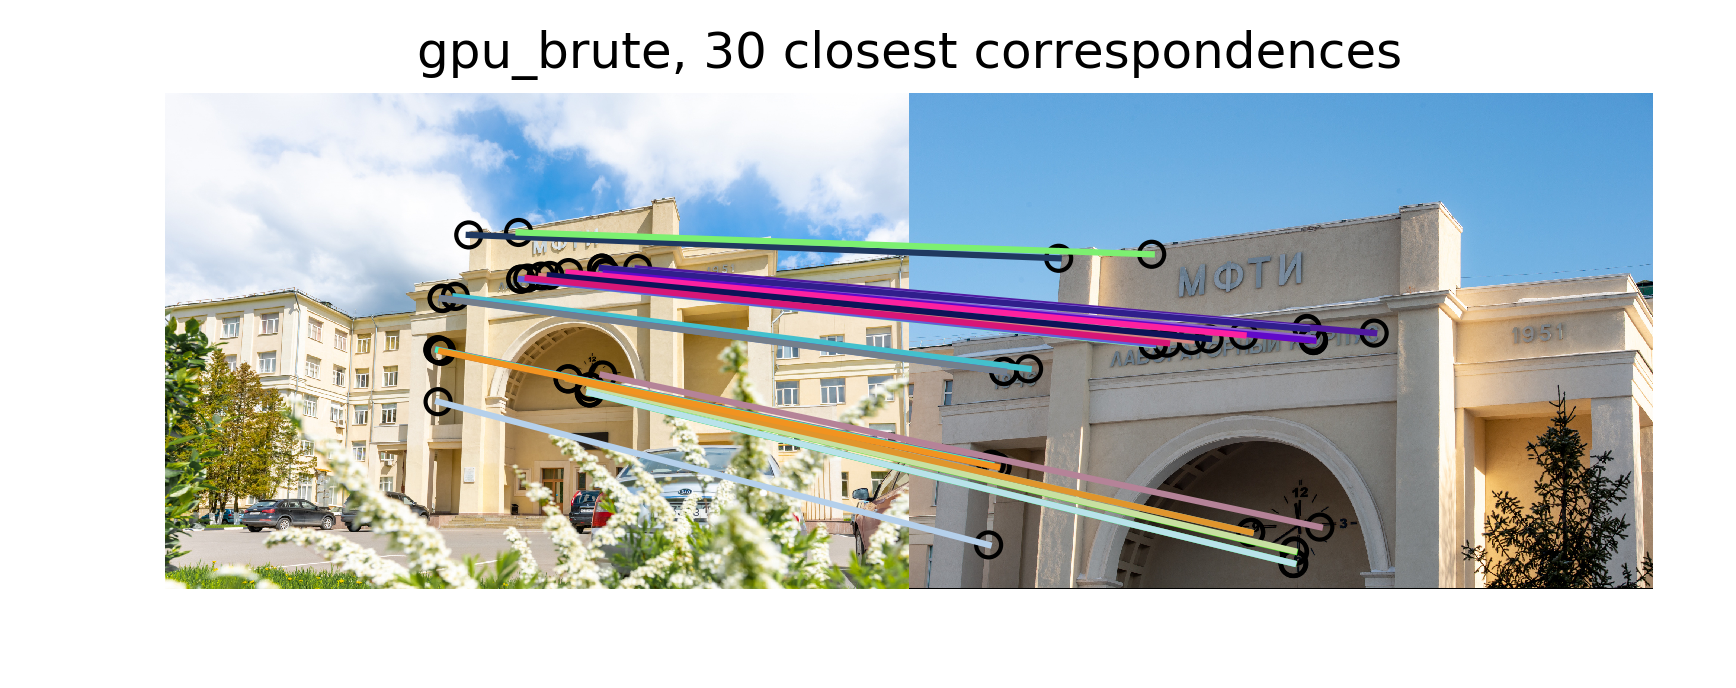
\includegraphics[width=\wid]{corresp_gpu_brute_4-5.png}
	\end{minipage}
	\hfill
	\begin{minipage}{\wid}
		
		%\caption{Time depending on algorithm/machine and query size}
		%\hspace{-1cm}
		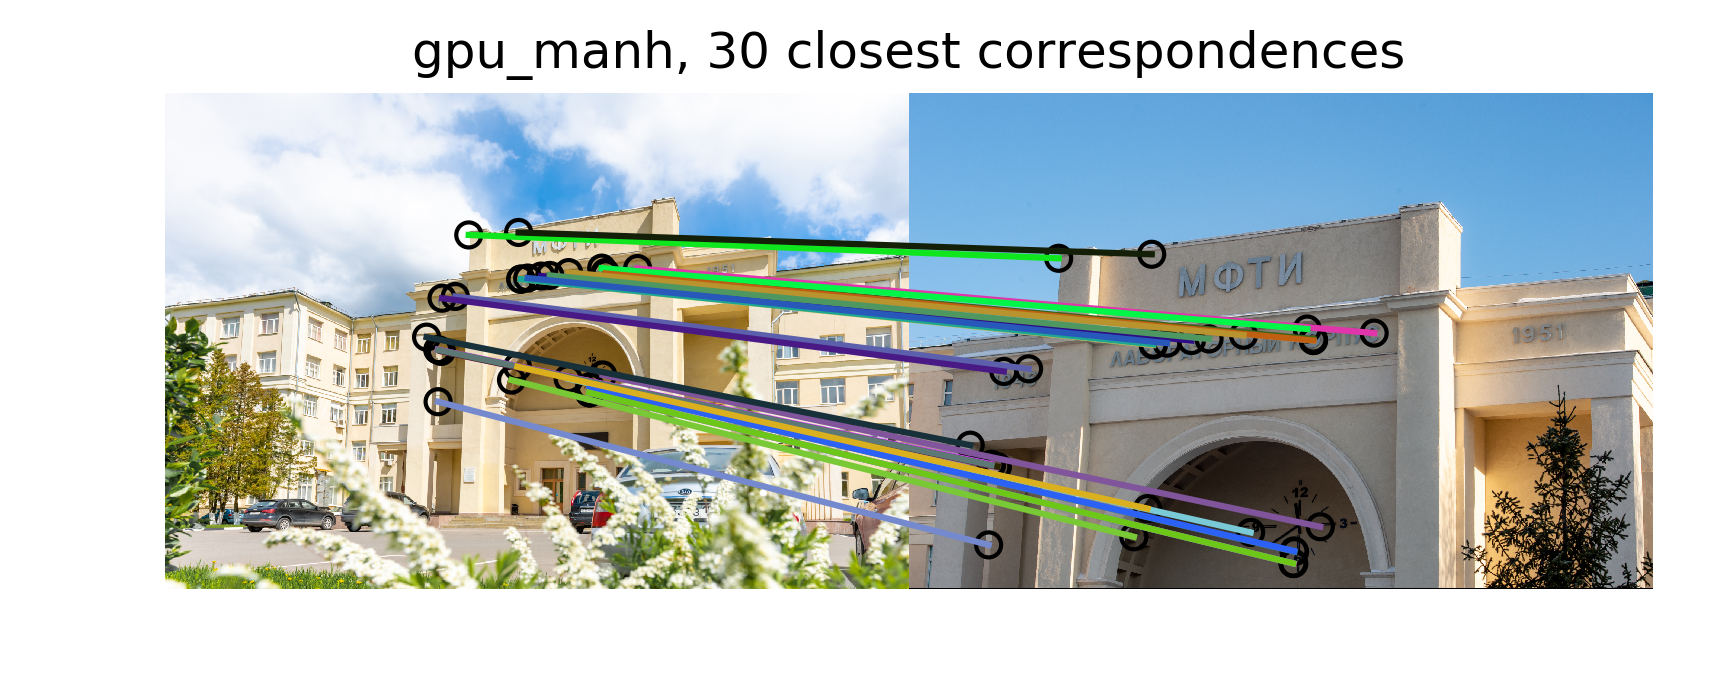
\includegraphics[width=\wid]{corresp_gpu_manh_4-5.png}
	\end{minipage}
	\hfill
	\begin{minipage}{\wid}
		
		%\caption{Time depending on algorithm/machine and query size}
		%\hspace{-1cm}
		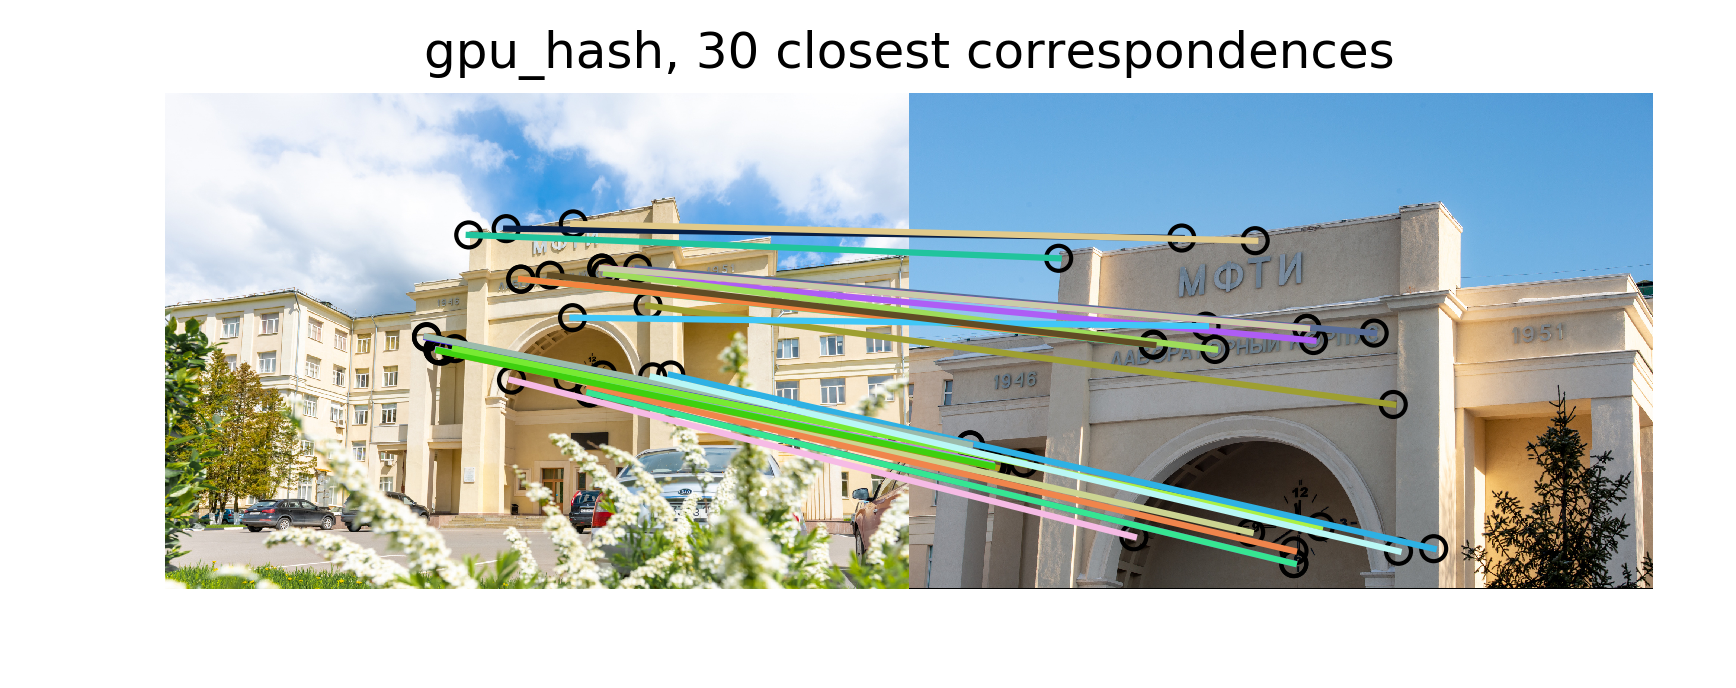
\includegraphics[width=\wid]{corresp_gpu_hash_4-5.png}
	\end{minipage}
\end{figure}
\end{frame}


\begin{frame}{How to find the best parameters? Which quality metric to use?}
\visible<1->{
	Metric of quality is the average Euclidean distance ("dist") in corresponding pairs.
	\begin{table}[]
		\begin{tabular}{|l|l|l|l|l|l|l|}
			\hline
			%\rowcolor[HTML]{ECF4FF} 
			\multirow{2}{*}{$t$, s} & \multirow{2}{*}{$\text{dist}$} & \multicolumn{4}{c|}{Parameters}\\ \cline{3-6}
			&& L & tableSize & M & W \\ \hline
			\textbf{0.496}   & \textbf{0.596} & \multicolumn{4}{l|}{ref. GPU brute--force}\\ \cline{1-6}
			0.492 & 0.602 & 3 & 17 & 1 & 0.5 \\
			0.443 & 0.624 & 3 & 37 & 1 & 0.1 \\
			0.254 & 0.654 & 1 & 83 & 3 & 0.5 \\
			0.172 & 0.678 & 1 & 83 & 3 & 0.1 \\ \hline
			
			
			
			
			
			
		\end{tabular}
		\caption {Example of dependence of results on the parameters of the method, for LSH}
	\end{table}
}
\end{frame}


\begin{frame}{Results for $N_{\text{query}} = 5000, N_{\text{db}} = 28188$}

\begin{table}[]
\hspace{1.5cm}
\begin{tabular}{|c|c|c|r|r|r|c|}
	\hline
	%\rowcolor[HTML]{ECF4FF} 
	Type & Mode & Av. dist & $t$, s &  \small $\text{std}(t)$, s & \small$\text{std(dist)}$ &  \small CPU/GPU\\ \hline
	
	\multirow{2}{*}{Brute-force}& CPU & \multirow{2}{*}{0.595} &  46.133 & 0.023 & 0 & \multirow{6}{*}{\textcolor{red}{$\sim80$}} \\ 
	& GPU & & 0.496 & 0.003 & 0  & \\ \cline{1-6}
	
	\multirow{2}{*}{Manhattan} & CPU & \multirow{2}{*}{0.608} & 24.632 & 2.585 & 0.066 & \\ 
	& GPU  & & 0.32 & 0.01 & 0.066 & \\ \cline{1-6}
	
	\multirow{2}{*}{LS Hashing} & CPU & \multirow{2}{*}{0.623} & 38.562  &2.077 & 0.066 &  \\ 
	& GPU &  & 0.439 & 0.006 & 0.066 & \\ \hline
\end{tabular}
\caption {Comparison of methods with the empirically best parameters}
\end{table}
"Best" taken parameters:\\
for Manhattan: $M=1, W=1$,\\
for LSH: $L=3, tableSize=83, M=1, W=0.1$.
\end{frame}

\begin{frame}[allowframebreaks]{References}
\printbibliography
\end{frame}

\end{document}
